\section*{ARGB representation of color%
\TAGS{bit-patterns}}

\enlargethispage{4ex}
In C0 we use 32-bit \lstinline'int's to represent a single
integer. However, it's possible to use the bits in other ways: as 32
separate Boolean values or as 4 separate 8-bit numbers in the range
$[0,255]$.  This lets us represent a color (red, green, and blue
intensities, plus transparency or ``alpha'') as an \lstinline'int':
\begin{center}
  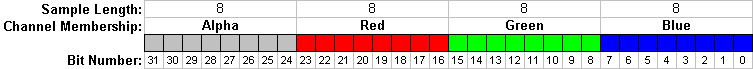
\includegraphics[width=\textwidth]{\img/PixelSamples32bppRGBA.png}
\end{center}
